\documentclass{zbc-report}

\usetikzlibrary{shapes.geometric}  % Including shapes.geometric for TikZ
\usepackage[normalem]{ulem}
\useunder{\uline}{\ul}{}

%% Set up the bibliography
\usepackage[backend=biber, style=apa]{biblatex}
\addbibresource{main.bib}

%% Additional packages and commands
\usepackage{parskip}
\setlist{itemsep=-2pt} % Reducing white space in lists slightly
\renewcommand{\deg}{\si{\degree}\xspace} % Use \deg easily, everywhere

%% Set up the graphics path
\usepackage{tikz}
\usetikzlibrary{angles, quotes, shapes.geometric, arrows.meta, positioning}
\tikzstyle{block} = [rectangle, rounded corners, minimum width=3cm, minimum height=1cm,text centered, draw=black, fill=blue!10]
\tikzstyle{arrow} = [thick, ->, >=Stealth]

%% Set up the minted package
\usepackage[cachedir=_minted-report]{minted}
\setminted{
    linenos=true,
    breaklines=true,
    fontsize=\footnotesize,
    frame=lines,
    framesep=2mm,
    baselinestretch=1.2,
    bgcolor=gray!10,
    style=vs,
    mathescape=true,
}

%% ----------------------------------------------------------------------
%%    Begin of document + Frontmatter (Roman page numbering)
%% ----------------------------------------------------------------------

\begin{document}

\frontmatter

%% Define the main parameters
\title{Synopsis}
\subtitle{AI and Machine Learning \\ 4. Semester}
\author{Carsten Lydeking}

\subject{Book recommender using NLP} % Cover only
\large\affiliation{Zealand Business College} % Cover only
\coverimage{figures/template-figures/binary.jpg} % Aspect ratio of 2:3 (portrait) recommended
\definecolor{title}{HTML}{4884d6} % Color for cover title

\makecover

\begin{titlepage}

\begin{center}

%% Print the title
{\makeatletter
\largetitlestyle\fontsize{45}{45}\selectfont\@title
\makeatother}

%% Print the subtitle
{\makeatletter
\ifdefvoid{\@subtitle}{}{\bigskip\titlestyle\fontsize{20}{20}\selectfont\@subtitle}
\makeatother}

\bigskip
\bigskip

%% Print the name of the author
{\makeatletter
\largetitlestyle\fontsize{25}{25}\selectfont\@author
\makeatother}

\bigskip
\bigskip

%% Print table with names and student numbers
\setlength\extrarowheight{2pt}
\begin{tabular}{c}
    cal002@edu.zealand.dk \\
\end{tabular}

\vfill

%% Print some more information at the bottom
\begin{tabular}{l r}
    Lecturer, AI and ML:   & Jens Peter Andersen \\
    Project Deadline: & \ddmmyydate{28/05/2025} \\
    Handed-in:       & \ddmmyydate{\today} \\
    Semester:        & 4. Semester\\
    Word Count:      & 23.460 Characters (including spaces) \\ %% Counted using texcount, not included in template
\end{tabular}

\bigskip
%% Add a source and description for the cover and optional attribution for the template
\begin{tabular}{l r}
    Cover: & Generated image of binary using DALL-E \\
    Style: & ZBC template -- created by Carsten Lydeking (Cally) \\
\end{tabular}


%% Insert the Zealand logo at the bottom of the page
\begin{tikzpicture}[remember picture]
    \node[above=10mm] at (current page.south) {%
        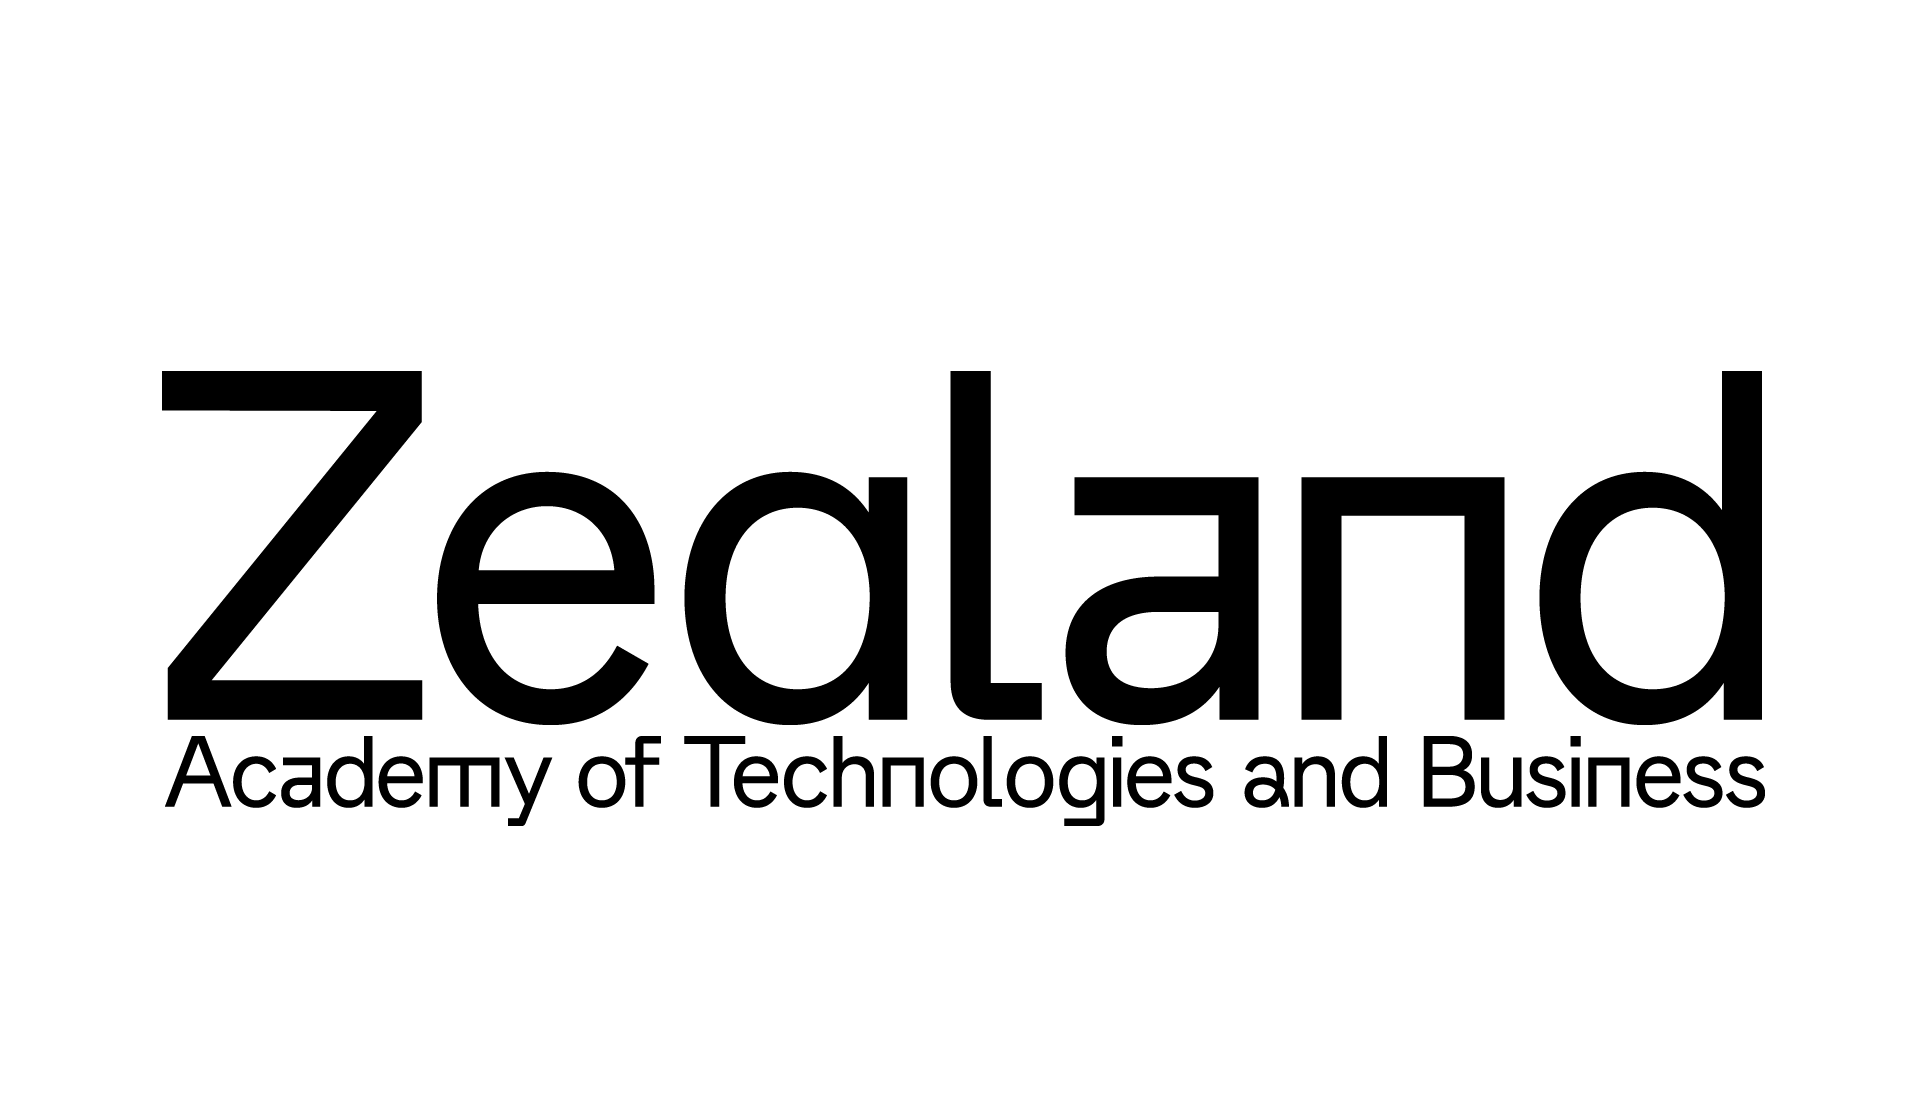
\includegraphics[width=0.35\textwidth]{figures/template-figures/zealandcombinedlogo}
    };
\end{tikzpicture}

\end{center}

\end{titlepage}

\tableofcontents
%\listoffigures
%\listoftables

%\chapter*{Nomenclature}
\addcontentsline{toc}{chapter}{Nomenclature}

\section{Abbreviations and definitions}
\label{sec:abbreviations}
The following abbreviations and definitions are used throughout the report:

\renewcommand{\arraystretch}{2}
\begin{longtable}{l p{13.5cm}}
    \textbf{Abb.}  & \textbf{Definition}  \\ \hline
        DB           & Database: A structured collection of data stored electronically. \\ \hline
        RDB          & Relational Database: A type of DB that stores and provides access to data points that are related to one another. \\ \hline
        DBMS         & Database Management System: Software that handles the storage, retrieval, and updating of data in a database. \\ \hline
        RDBMS        & Relational DBMS: A database management system based on the relational model introduced by E.F. Codd. \\ \hline
        SQL          & Structured Query Language: A programming language used to manage and manipulate relational databases. \\ \hline
        CRUD         & Create, Read, Update, Delete The four basic operations of persistent storage: adding, retrieving, modifying, and removing data. \\ \hline
        GUI          & Graphical User Interface  A user interface that allows users to interact with electronic devices using graphical icons and visual indicators. \\ \hline
        PK           & Primary Key:A unique identifier for each record in a database table. \\ \hline
        FK           & Foreign Key: A field in a database table that links to the primary key of another table. \\ \hline
        NML          & Normalization: In relation to RDB design, the process of organizing the columns (attributes) and tables (relations) to minimize data redundancy. \\ \hline
        1NF          & First Normal Form: A stage of NML where each table has atomic (i.e. indivisible) values and each record needs to be unique. \\ \hline
        2NF          & Second Normal Form: A stage of NML where it meets all the requirements of the 1NF and does not have partial dependency. \\ \hline
        3NF          & Third Normal Form: A stage of NML where it meets all the requirements of the 2NF and has no transitive functional dependencies. \\ \hline
        ERD          & Entity Relationship Diagram: A graphical representation of entities and their relationships to each other, typically used in database design. \\ \hline
        UML          & Unified Modeling Language: A standardized modeling language used to specify, visualize, construct, and document the artifacts of software systems. \\ \hline
        DDL          & Data Definition Language: A subset of SQL used to define database structures, such as tables, schemas, and databases. \\ \hline
        DML          & Data Manipulation Language: A subset of SQL used for adding (inserting), deleting, and modifying (updating) data in a database. \\ \hline
        DCL          & Data Control Language: A subset of SQL used to control access to data in a database. \\ \hline
        TCL          & Transaction Control Language: A subset of SQL used to manage the changes made by DML statements. \\ \hline
        XML          & Extensible Markup Language: A markup language that defines a set of rules for encoding documents in a format that is both human-readable and machine-readable. \\ \hline
        JSON         & JavaScript Object Notation: A lightweight data-interchange format that is easy for humans to read and write, and for machines to parse and generate. \\ \hline
    \renewcommand{\arraystretch}{1}
\end{longtable}

%% ----------------------------------------------------------------------
%%    Mainmatter (Arabic page numbering)
%% ----------------------------------------------------------------------

\mainmatter

\chapter{Introduction}
\label{chapter:introduction}

\section{Motivation}
\label{sec:motivation}

This project explores the feasibility of deploying local machine learning models for intelligent information retrieval in local environments. 
As a case study, a fully local book recommendation system is developed. 
It leverages Natural Language Processing (NLP) techniques to analyze both book descriptions and natural language queries from users, enabling semantically meaningful, content-based recommendations.

In contrast to cloud-based systems that depend on centralized APIs and remote computation, this solution demonstrates a standalone, offline setup. 
All data processing — including text embedding, category inference, indexing, and query resolution — occurs on the user’s device, ensuring that no personal data leaves the local environment.

The core goal is to evaluate whether lightweight transformer-based models, specifically sentence transformers like MiniLM, can provide reliable and personalized recommendations within such constraints. 
The system incorporates semantic embedding, category inference through zero-shot classification, vector similarity search via FAISS, and Streamlit interface. 
These components collectively address the broader question of how accessible and effective locally hosted AI tools can be for individual users.

\section{Problem Definition}
\label{sec:problem-definition}

The project is centered around the following research question:

\begin{quote}
\textit{How can a local ML model be used to recommend books based on natural language descriptions, relying only on locally running models?}
\end{quote}

This leads to three guiding sub-questions:

\begin{enumerate}
    \item \label{itm:subq-embedding} \textit{What techniques exist for embedding text into meaningful vectors?}
    \item \label{itm:subq-similarity} \textit{How can vector similarity be used for finding relevant books?}
    \item \label{itm:subq-classification} \textit{How can genre categories be inferred and used to improve indexing and filtering?}
    \item \label{itm:subq-limitations} \textit{What are the practical limitations of a local, content-only recommendation system?}
\end{enumerate}

These sub-questions form the conceptual framework for the analysis presented throughout the synopsis.

\section{Link to code repository}
The code is public on GitHub: \href{https://github.com/Cal-ly/LLM-Book-Recommender}{\textit{https://github.com/Cal-ly/LLM-Book-Recommender}}.

\chapter{Methodology and Structure}
\label{chapter:methodology}

This project follows a research-based prototype methodology. 
Rather than developing a commercial software product, the goal is to explore the scientific and 
technical feasibility of running semantic book recommendations using local machine learning tools.
The findings—both theoretical and experimental—constitute the core deliverables of this project.

\section{Research Approach}
\label{sec:research-approach}

The project is based on a combination of literature review and hands-on implementation. 
Each aspect of the methodology was selected to support answering the sub-questions defined in Section~\ref{sec:problem-definition}.

\begin{itemize}
    \item \textbf{Literature Review:} Relevant topics included natural language processing (NLP), sentence embedding techniques, 
    recommender systems, and similarity search. Key technologies such as \texttt{MiniLM}, \texttt{FAISS}, 
    and \texttt{Streamlit} were studied through documentation and other sources. As this field is rapidly evolving,
    the latest knowledge regarding pracitcal applications was prioritized, e.g. \cite{handson-ml}.
    
    \item \textbf{Implementation:} The following tools and libraries were used throughout the project:
    \begin{itemize}
        \item \texttt{Python} for scripting, preprocessing, and experimentation.
        \item \texttt{pandas}, \texttt{seaborn}, and \texttt{matplotlib} for data analysis and visualization.
        \item \texttt{sentence-transformers} (MiniLM-L6-v2) to generate semantic vector representations.
        \item \texttt{FAISS} to index and search high-dimensional embeddings efficiently.
        \item \texttt{Streamlit} to build an interactive, privacy-preserving user interface.
    \end{itemize}
    
    \item \textbf{Testing:} Practical testing included a range of user queries and filtering conditions to observe whether recommendations matched the query intent semantically.
\end{itemize}

---

\section{Evaluation Criteria}
\label{sec:evaluation-criteria}

As no supervised training or labeled ground-truth data was involved, the system is evaluated using non-traditional metrics. The following criteria were applied:

\begin{itemize}
    \item \textbf{Qualitative Relevance:} Whether the recommendations appear semantically relevant to a human evaluator.
    \item \textbf{Responsiveness:} How quickly the system responds to user queries on consumer hardware.
    \item \textbf{Offline Capability:} Verification that all processing occurs locally, without internet access.
    \item \textbf{Scalability:} Exploration of performance with larger datasets and indexing sizes.
\end{itemize}

This methodology supports the central research question posed in \autoref{itm:main-question}, and particularly sub-questions~\ref{itm:subq-embedding} and~\ref{itm:subq-similarity}, by grounding each system component in both theoretical research and empirical testing.

---

\section{Structure of the Synopsis}
\label{sec:structure-synopsis}
The synopsis is structured with each chapter addressing a specific aspect of the project and each chapter builds upon the previous one to provide an overview of the project.
\subsection{Main Chapters}
\begin{itemize}
    \item \cref{chapter:introduction} introduces the motivation, problem definition, and research approach.
    \item \cref{chapter:methodology} describes the research methodology and evaluation criteria.
    \item \cref{chapter:dataset} explores the dataset used, including its cleaning and preprocessing. 
    \item \cref{chapter:embedding} covers the embedding process, including the theory and implementation of sentence embeddings. 
    \item \cref{chapter:similarity} describes the FAISS indexing and similarity search process.
    \item \cref{chapter:interface} describes the user interface design and query workflow.
    \item \cref{chapter:performance} discusses the performance evaluation and challenges of the system, including qualitative and quantitative metrics.
    \item \cref{chapter:conclusion} discusses the results, limitations, and future work.
\end{itemize}

\subsection{Appendices}
A deeper dive into the technical details of the implementation is provided in the appendices, including a more theoretical background on both ML and mathematical concepts.
This has been deliberately kept separate from the main chapters, as the focus of the synopsis is on the practical application and results rather than the underlying theory.

---

\section{Application Architecture}
\label{sec:application-architecture}
The architecture of the book recommendation system:

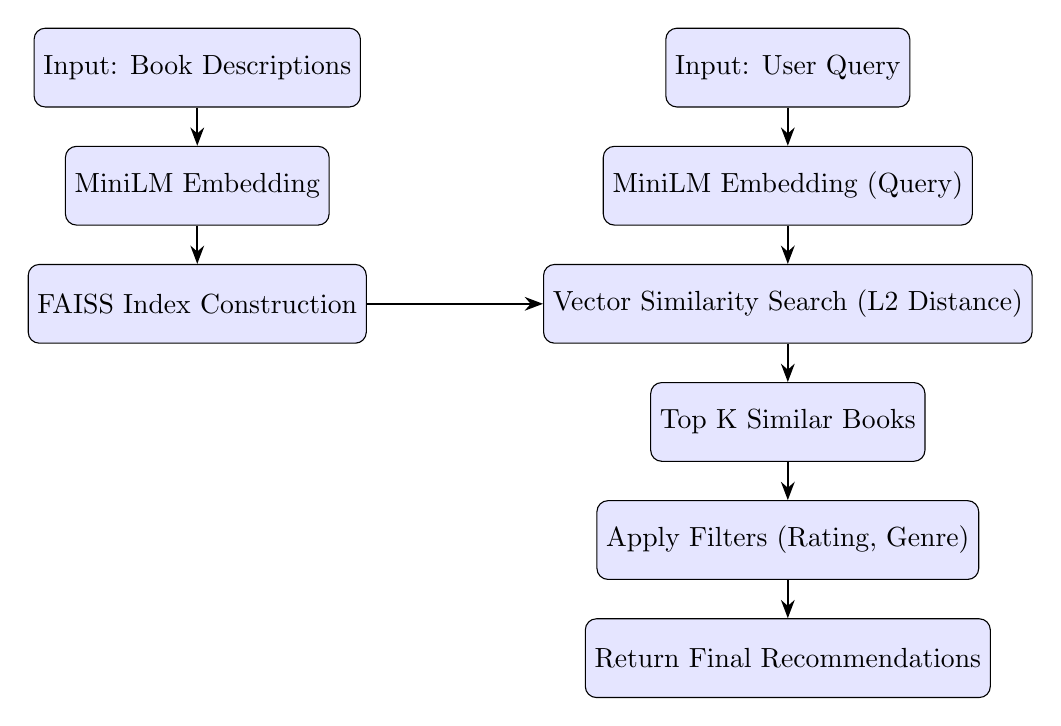
\begin{tikzpicture}[node distance=1.5cm]

    \node (desc) [block] {Input: Book Descriptions};
    \node (minilm) [block, below of=desc] {MiniLM Embedding};
    \node (index) [block, below of=minilm] {FAISS Index Construction};
    
    \node (query) [block, right of=desc, xshift=6cm] {Input: User Query};
    \node (qembed) [block, below of=query] {MiniLM Embedding (Query)};
    \node (simsearch) [block, below of=qembed] {Vector Similarity Search (L2 Distance)};
    
    \node (topk) [block, below of=simsearch] {Top K Similar Books};
    \node (filter) [block, below of=topk] {Apply Filters (Rating, Genre)};
    \node (output) [block, below of=filter] {Return Final Recommendations};
    
    % Arrows
    \draw [arrow] (desc) -- (minilm);
    \draw [arrow] (minilm) -- (index);
    \draw [arrow] (query) -- (qembed);
    \draw [arrow] (qembed) -- (simsearch);
    \draw [arrow] (index) -- (simsearch);
    \draw [arrow] (simsearch) -- (topk);
    \draw [arrow] (topk) -- (filter);
    \draw [arrow] (filter) -- (output);
    
\end{tikzpicture}
\chapter{Dataset Exploration}
\label{chapter:dataset}

The project began with the public dataset by Castillo (2025), containing metadata for over 6,800 books. Initial inspection revealed missing or inconsistent fields such as authorship, categories, and descriptions. A modular preprocessing pipeline was built to clean, augment, and prepare the data for semantic modeling.

\section{Dataset Overview}
The original dataset (\texttt{books.csv}) included fields such as:
\begin{itemize}
\item \verb|isbn13|, \verb|title|, \verb|subtitle|, \verb|authors|
\item \verb|categories|, \verb|description|, \verb|published_year|
\item \verb|average_rating|, \verb|num_pages|
\end{itemize}
Key fields were combined and engineered into a unified \verb|full_title|, and several boolean \verb|has_*| flags were created for inspection and filtering.

\section{Data Cleaning and Augmentation}
Cleaning and augmentation were performed in multiple stages:
\begin{enumerate}
\item \textbf{Initial Checks:} Detected and logged missing or invalid entries.
\item \textbf{OpenLibrary Augmentation:} Filled in missing values such as \texttt{authors}, \texttt{num\_pages}, and \texttt{thumbnail}. Introduced \texttt{subjects}.
\item \textbf{Google Books API:} Prioritized short or missing descriptions and added alternate fields (e.g., \texttt{description\_google}).
\item \textbf{Field Comparison:} Logged mismatches in fields like title and author between sources. Created \texttt{alt\_*} fields where minor but significant discrepancies were found.
\item \textbf{Final Merging:} Consolidated \texttt{categories}, \texttt{subjects}, and \texttt{categories\_google} into a cleaned \texttt{final\_categories} field.
\end{enumerate}
Records with less than 9 words in the final description were removed, reducing the dataset from 6,810 to 6,572 entries.

\section{Feature Engineering}
New fields were engineered to support classification and filtering:
\begin{itemize}
\item \verb|words_in_description| \textemdash{} token count of description
\item \verb|description_length| \textemdash{} character count of enriched description
\item \verb|has_*| flags \textemdash{} completeness indicators for filtering
\end{itemize}
These were used both for data readiness assessments and visualization.

\section{Exploratory Analysis}
Visual and statistical analysis was used to inform thresholds and highlight data issues:
\begin{itemize}
\item \textbf{Missing Values:} \verb|openlib_values_heatmap.png|
\item \textbf{Rating Distribution:} \verb|rating_distribution.png|
\item \textbf{Publication Year:} \verb|publication_year_distribution.png|
\item \textbf{Category Frequency:} \verb|top_categories.png|
\item \textbf{Short Descriptions:} \verb|less_than_50_words_description.png|
\item \textbf{Metadata Conflicts:} \verb|reexp_mismatch_counts.png|
\end{itemize}
These figures helped guide filtering strategies and offered insight into metadata quality.

\section{Outcome}
After augmentation and filtering, 6,572 books remained. These were passed to the category inference pipeline (Chapter~\ref{chapter:category-inference}), where further refinement reduced the set to 5,160 high-confidence entries suitable for semantic embedding and indexing.
\chapter{Category Inference}
\label{chapter:category-inference}

To support genre-aware filtering and embedding, each book in the dataset is automatically labeled with one or more thematic categories. 
This process combines transformer-based zero-shot classification with a curated keyword-based fallback strategy, confidence-based filtering, and semantic cleaning. The refined categories are ultimately used for filtering, indexing, and interface interaction.

\section{Zero-Shot Classification with BART-MNLI}
Each book is first enriched with an \texttt{augmented\_description} field, combining its full title, author, publication year, and description. 
These are then fed into a zero-shot classification model, \texttt{facebook/bart-large-mnli} \cite{bart-large-mnli}, using Hugging Face’s \texttt{pipeline} for multi-label inference across 13 candidate categories (e.g. \textit{Fantasy}, \textit{Love}, \textit{Non-fiction}).

Predictions below a confidence threshold of 0.4 are discarded. Each book retains only the labels with strong relevance, based on model probabilities.

\section{Fallback Keyword Enrichment}
To improve recall and thematic depth, fallback keywords are used when the model fails to detect relevant categories. 
Each category has a corresponding keyword list (e.g. \texttt{“magic”}, \texttt{“orc”}, \texttt{“griffin”} for \textit{Fantasy}; \texttt{“vampire”}, \texttt{“haunted”}, \texttt{“exorcism”} for \textit{Horror}).

Fallback labels are only added if the model’s predictions do not already include them. In total, fallback logic affected 4665 out of 6572 rows.

\section{Refinement, Merging, and Metrics}
To reduce redundancy and overlap, closely related categories are merged:
\begin{itemize}
  \item \textbf{Biography + History} $\rightarrow$ \textit{Historical}
  \item \textbf{Philosophy + Poetry} $\rightarrow$ \textit{Philosophy \& Poetry}
  \item \textbf{Suspense + Detective} $\rightarrow$ \textit{Mystery}
\end{itemize}

Per-category precision, recall, and F1 scores are calculated using known metadata labels for validation. Visualizations and metric CSVs are generated for review.

\section{Confidence Analysis and Filtering}
Each row is evaluated using the following confidence metrics:
\begin{itemize}
  \item \texttt{max\_score}: Highest label confidence
  \item \texttt{filtered\_avg\_score}: Average score excluding labels under 0.2
  \item \texttt{score\_std}: Standard deviation across all label scores
  \item \texttt{num\_categories}: Total confident categories retained
\end{itemize}

To prepare for indexing, only rows satisfying all of the following are retained:
\begin{itemize}
  \item Description length $\geq$ 200 characters
  \item \texttt{filtered\_avg\_score} $\geq$ 0.2
  \item \texttt{max\_score} $\geq$ 0.4
  \item At least one confident category
\end{itemize}

This reduced the dataset from 6572 to 5160 books.

\section{Length vs Confidence Correlation}
To verify the impact of text richness, correlation between \texttt{description\_length} and \texttt{average\_score} was analyzed. The results:

\begin{itemize}
  \item Pearson correlation: $r=0.398$ ($p<0.0001$)
  \item Spearman rank: $\rho=0.261$ ($p<0.0001$)
\end{itemize}

This indicates a moderate positive relationship between description length and model confidence, validating the filtering step as both qualitative and statistically grounded.

\chapter{Text Embedding}
\label{chapter:embedding}

The core of the recommendation system lies in transforming books and queries into a shared semantic space. 
This is accomplished by generating sentence embeddings that encode the meaning of input text into numerical vectors. Once embedded, semantic similarity can be computed between queries and books.

\section{Sentence Embedding Theory}
\label{sec:embedding-theory}

Sentence embeddings are dense vector representations of variable-length text sequences. 
They enable comparison of textual content by mapping semantically similar sentences to nearby points in vector space. The process relies on transformer-based models.

Let $f(t)$ be the embedding function applied to a string $t$, producing a vector $\vec{v} \in \mathbb{R}^{384}$:
\begin{equation}
\vec{v} = f(t), \quad \vec{v} \in \mathbb{R}^{384}
\end{equation}

This project uses \texttt{all-MiniLM-L6-v2} from the Hugging Face \texttt{sentence-transformers} library, which produces 384-dimensional embeddings. 
It offers an excellent balance between speed and semantic quality, making it ideal for offline inference on CPU hardware.

\section{Embedding Implementation}
\label{sec:embedding-implementation}

Text embeddings were generated using a composite string field \texttt{search\_text}, constructed for each book as follows:

\begin{verbatim}
Title: {full_title}. Author: {authors}. Description: {description}
\end{verbatim}

This format ensures that both metadata and narrative content contribute to the semantic embedding. The following steps were performed:
\begin{enumerate}
    \item Loaded the final dataset \texttt{books\_indexed.csv}.
    \item Encoded each \texttt{search\_text} entry using MiniLM.
    \item Saved the resulting matrix of shape $(n, 384)$ to memory.
    \item Added all vectors to a FAISS index (see Chapter~\ref{chapter:faiss}).
    \item Saved metadata with vectors to \texttt{books\_indexed\_with\_embeddings.csv}.
\end{enumerate}

\section{Embedding Configuration}
\label{sec:embedding-config}

The embedding stage used the following parameters:
\begin{itemize}
    \item \textbf{Model:} \texttt{all-MiniLM-L6-v2}
    \item \textbf{Library:} \texttt{sentence-transformers}
    \item \textbf{Embedding Dimension:} 384
    \item \textbf{Distance Metric:} L2 (Euclidean)
    \item \textbf{Backend:} CPU inference
    \item \textbf{Input Field:} \texttt{search\_text}
    \item \textbf{Entries Embedded:} 5,160 books
\end{itemize}

\section{Summary}
\label{sec:embedding-summary}

The embedding pipeline enabled semantic similarity computations between books and queries. Using a compact transformer model, each entry was encoded into a vector capturing its latent meaning. 
This allowed content-based querying without relying on metadata fields like genre, author popularity, or user behavior. The resulting vectors were stored in a FAISS index for efficient similarity search.

\chapter{Vector Similarity Search with FAISS}
\label{chapter:faiss}

Once books and queries are embedded into the same semantic space, the system must identify the most relevant books for a given user input. This is achieved using vector similarity search. In this project, the FAISS (Facebook AI Similarity Search) library is used to enable fast and accurate nearest-neighbor retrieval over the 5,160 book vectors.

\section{Similarity Search Theory}
\label{sec:similarity-theory}

Let \( \vec{q} \in \mathbb{R}^{384} \) represent the embedded user query, and let \( \{\vec{b}_1, \vec{b}_2, \dots, \vec{b}_n\} \) denote the embedded book vectors. The similarity between the query and each book is computed using squared L2 (Euclidean) distance:

\begin{equation}
    \text{dist}(\vec{q}, \vec{b}_i) = \|\vec{q} - \vec{b}_i\|_2^2
\end{equation}

The top \( k \) nearest neighbors (i.e., those with the smallest distances) are returned as recommended books. This approach assumes that semantically similar texts lie close together in vector space.

\section{Why FAISS?}
\label{sec:faiss-choice}

FAISS is optimized for fast similarity search over high-dimensional vectors. It was selected for this project because it:

\begin{itemize}
    \item \textbf{Performs well on CPU} — fast enough for real-time use
    \item \textbf{Supports exact and approximate search} — adaptable for scale
    \item \textbf{Offers simple integration with NumPy and PyTorch}
    \item \textbf{Runs offline} — no internet connection required
\end{itemize}

This implementation uses \texttt{IndexFlatL2}, a brute-force index that performs exact nearest-neighbor search using squared L2 distance. It is suitable for small to medium datasets and does not require tuning.

\section{Implementation}
\label{sec:similarity-implementation}

After the embeddings were generated (see Chapter~\ref{chapter:embedding}), the similarity search process was implemented as follows:

\begin{enumerate}
    \item Initialize a \texttt{faiss.IndexFlatL2} index with vector dimension 384.
    \item Add the 5,160 book vectors to the index.
    \item At runtime:
    \begin{itemize}
        \item Embed the user query using the same MiniLM model.
        \item Use FAISS to find the top \( k \) nearest book vectors.
        \item Retrieve metadata from \texttt{books\_indexed\_with\_embeddings.csv}.
    \end{itemize}
\end{enumerate}

The system achieves sub-second response times on consumer-grade laptops using only CPU.

\section{Summary}
\label{sec:similarity-summary}

FAISS powers the core similarity engine of the recommender system. Combined with MiniLM embeddings, it enables local, real-time, and semantically aware recommendations. The entire matching process relies solely on content, requiring no user profiles or interaction history.

\chapter{User Interface}
\label{chapter:interface}

The user interface enables interaction with the semantic book recommendation system. 
While not a machine learning component, it plays a crucial role in usability, filtering, and presentation. 
The interface is implemented using \texttt{Streamlit}, a lightweight Python framework suitable for local-first applications.

\section{Design Principles}
\label{sec:ui-design}

The UI was designed with simplicity and responsiveness in mind. It supports end-to-end offline operation. Design goals included:

\begin{itemize}
    \item Concept-based natural language search
    \item Multi-faceted filtering by category and rating
    \item Minimal dependencies and fast startup
    \item Clear presentation of recommendations
\end{itemize}

All inference and retrieval logic runs locally.

\section{Query Workflow}
\label{sec:ui-query-workflow}

The system accepts a free-form text query from the user (e.g., \textit{``Books about surviving on Mars''}). The workflow proceeds as follows:

\begin{enumerate}
    \item Query is embedded using the MiniLM model.
    \item The FAISS index returns the top 60 nearest book vectors.
    \item Filtering and sorting options are applied.
    \item Six book cards are rendered per page.
\end{enumerate}

This approach allows expressive, language-based search.

\section{Filtering and Sorting}
\label{sec:ui-filtering}

Users can refine results with:

\begin{itemize}
    \item \textbf{Category filter:} Multi-select widget for genre labels
    \item \textbf{Rating sort:} Toggle for ascending/descending order
    \item \textbf{Pagination:} Adjustable page selection for navigation
\end{itemize}

Filters are applied after FAISS similarity search.

\section{Result Display}
\label{sec:ui-display}

Each result is rendered as a card containing:

\begin{itemize}
    \item Book cover image (URL with fallback)
    \item Full title and author
    \item Average rating, number of pages, and publication year
    \item Description excerpt (up to 300 characters)
    \item Refined categories
\end{itemize}

The layout ensures readability and intuitive navigation.

\section{Privacy and Offline Execution}
\label{sec:ui-privacy}

The application is designed for full offline use:

\begin{itemize}
    \item No tracking, cookies, or login
    \item No data transmission to external servers
    \item Book data, models, and index are stored locally
\end{itemize}

This ensures data privacy, fast load times, and compatibility with low-resource environments.

\section{Summary}
\label{sec:ui-summary}

The Streamlit interface allows users to interact with the system seamlessly. 
Natural language search, combined with real-time filtering and semantic recommendations, creates an intuitive and private discovery experience.
\chapter{Performance and Evaluation Challenges}
\label{chapter:performance}

This chapter outlines how the system’s performance was evaluated, given the absence of user feedback and labeled test data. Traditional metrics such as accuracy or precision are not directly applicable to semantic similarity tasks without ground truth. Therefore, evaluation is divided into subjective, statistical, and system-level components.

\section{Evaluation Without Labels}
\label{sec:no-labels}

The system does not predict a fixed label or class. Instead, it embeds both queries and books in a shared vector space and retrieves nearest neighbors using semantic distance. As a result:

\begin{itemize}
    \item There is no single “correct” recommendation per query.
    \item Precision/recall-based metrics cannot be used reliably.
    \item Feedback mechanisms like click-through or engagement data are unavailable in an offline setting.
\end{itemize}

This necessitates alternative evaluation strategies.

\section{Qualitative Evaluation}
\label{sec:qualitative-eval}

Evaluation relied on exploratory queries and manual inspection of results. Test queries covered a range of genres, tones, and abstraction levels. Examples include:

\begin{itemize}
    \item ``Existential loneliness in space''
    \item ``Post-apocalyptic survival story''
    \item ``Books that explore grief through fantasy''
\end{itemize}

Results were judged based on alignment between the query and the content of the returned book descriptions. This human-in-the-loop approach confirmed that semantically aligned results were typically returned.

\section{Category Inference Evaluation}
\label{sec:category-eval}

Although the original dataset lacked consistent genre labels, the quality of inferred categories was assessed via:

\begin{itemize}
    \item Retaining classification confidence scores per label
    \item Filtering by a threshold of 0.4 (see Chapter~\ref{chapter:categories})
    \item Computing precision, recall, and F1 scores for a subset of trusted entries
    \item Visualizing match counts and fallback coverage
\end{itemize}

Certain categories (e.g., \textit{Fantasy}, \textit{Love}) were strongly predicted by the model, while others (e.g., \textit{Philosophy \& Poetry}) relied more heavily on fallback keyword enrichment.

\section{Responsiveness and Latency}
\label{sec:latency}

Performance was measured on a consumer-grade laptop (no GPU):

\begin{itemize}
    \item Query embedding time (MiniLM): $< 0.2$ seconds
    \item FAISS top-60 vector search: $< 10$ ms
    \item Streamlit UI rendering (6 cards per page): $< 2$ seconds including image fallback
\end{itemize}

This confirms that the system operates in real time on modest hardware, supporting its offline-first goal.

\section{Scalability Considerations}
\label{sec:scaling}

While the current dataset (5,160 entries) is manageable, scaling raises practical challenges:

\begin{itemize}
    \item \textbf{Indexing:} FAISS IndexFlatL2 is efficient but linear in search time; approximate methods (e.g., HNSW) may be needed for larger corpora.
    \item \textbf{Re-embedding:} Changing models or descriptions requires recomputing all embeddings.
    \item \textbf{Filtering:} UI-side filtering and sorting scale linearly with post-search result volume.
\end{itemize}

Future extensions should consider vector compression, batch processing, and caching.

\section{Limitations of Offline Evaluation}
\label{sec:limitations}

Offline evaluation limits the types of insights that can be gathered:

\begin{itemize}
    \item \textbf{Relevance:} Relies solely on developer judgment
    \item \textbf{Discovery:} Cannot measure novelty or serendipity
    \item \textbf{Bias Detection:} Overrepresentation of certain authors or genres may go unnoticed
\end{itemize}

These are acceptable trade-offs in the context of a local, user-respecting prototype.

\section{Summary}
\label{sec:performance-summary}

Evaluation focused on semantic quality, practical responsiveness, and offline usability. Despite the lack of supervised benchmarks, confidence filtering, manual validation, and runtime measurements demonstrated that the system is performant and aligned with its design goals.

\chapter{Conclusion}
\label{chapter:conclusion}

This chapter summarizes the findings and outcomes of the project, reflects on its limitations, and revisits the original research questions.

\section{Discussion}
\label{sec:discussion}

This project demonstrated that transformer-based models can power a local, content-only book recommendation system. Without requiring user profiles or collaborative filtering, the system delivers semantically meaningful recommendations based entirely on book metadata and free-text queries.

The end-to-end system consisted of:
\begin{itemize}
    \item Augmented and cleaned metadata for over 6,800 books
    \item Zero-shot genre inference using BART-MNLI with fallback keyword enrichment
    \item Semantic embeddings via MiniLM
    \item FAISS-based vector search
    \item A responsive, private UI implemented in Streamlit
\end{itemize}

With no reliance on internet access, the system runs entirely offline and respects user privacy. It is suitable for low-resource environments and educational use cases.

\section{Conclusion}
\label{sec:conclusion}

The system successfully addressed all four research sub-questions:

\begin{enumerate}
    \item \textbf{What techniques exist for embedding text into meaningful vectors?}  
    Pretrained sentence transformers like MiniLM encode text into high-dimensional semantic vectors, enabling rich similarity comparisons.

    \item \textbf{How can vector similarity be used for finding similar books?}  
    FAISS enables fast nearest-neighbor retrieval in vector space, allowing queries to return top-matching books based on content alone.

    \item \textbf{How can genre categories be inferred and used for filtering?}  
    BART-MNLI enables zero-shot classification of genre labels. Fallback keyword rules and confidence filtering improve label coverage and reliability.

    \item \textbf{What are the limitations of a local, content-only recommender?}  
    The system lacks personalization and behavior-driven refinement. However, it compensates with transparency, offline execution, and semantic precision.
\end{enumerate}

\noindent
\textbf{Main research question:}

\begin{quote}
\textit{How can a local ML model be used to recommend books based on natural language descriptions, relying only on locally running models?}
\end{quote}

This was answered by developing and validating a fully local recommendation system that performs semantic classification, embedding, indexing, and retrieval — all on-device.

\section{Reflection}
\label{sec:reflection}

The project offered valuable insights into building ML-powered applications under strict resource constraints. Key lessons include:

\begin{itemize}
    \item \textbf{Description quality drives results:} Well-written descriptions significantly enhance semantic accuracy.
    \item \textbf{Fallbacks expand coverage:} Keyword-based strategies improve classification when the model lacks confidence.
    \item \textbf{Local-first ML is viable:} Even compact transformer models provide robust performance on consumer hardware.
    \item \textbf{Simplicity over complexity:} Lightweight, modular design reduced failure points and increased maintainability.
\end{itemize}

With more time, the system could be extended to include:

\begin{itemize}
    \item Comparison of embedding models (e.g., MPNet, SBERT)
    \item Re-ranking of results based on metadata
    \item Interactive user feedback or offline learning
\end{itemize}

The project demonstrates that privacy-respecting, offline-first NLP systems are not only possible but practical. This aligns with emerging interest in edge-based AI and user-sovereign computing.
In a forward-looking perspective, the system could serve as a foundation for more complex applications - such as personalized learning assistants or local knowledge bases - 
further enhancing the utility of AI in everyday life while respecting user privacy.


%% Prevent urls running into margins in bibliography
\setcounter{biburlnumpenalty}{7000}
\setcounter{biburllcpenalty}{7000}
\setcounter{biburlucpenalty}{7000}

%% Add bibliography
\printbibliography[heading=bibintoc,title={References}]

%% ----------------------------------------------------------------------
%%    Appendix (Letters for chapters)
%% ----------------------------------------------------------------------

\appendix

% Glossaries
\appendix
\chapter{Glossary of Mathematical Symbols}
\label{appendix:symbols}

This glossary defines the mathematical symbols used throughout the theory and math appendices.

\section*{General Symbols}

\begin{tabular}{lp{10cm}}
    $\mathbb{R}$ & The set of real numbers \\
    $n$ & Number of entries (e.g., books or documents) \\
    $d$ & Dimensionality of embedding space (e.g., 384) \\
    $i$ & Index of an individual book or word \\
\end{tabular}

\vspace{1em}

---

\section*{Vectors and Embeddings}

\begin{tabular}{lp{10cm}}
    $\vec{v}$ & General vector (e.g., sentence embedding) \\
    $\vec{q}$ & Query vector (user input) \\
    $\vec{b}_i$ & Embedding of the $i$th book \\
    $\|\vec{v}\|_2$ & L2 (Euclidean) norm or length of vector $\vec{v}$ \\
    $\vec{a} \cdot \vec{b}$ & Dot product between vectors $\vec{a}$ and $\vec{b}$ \\
    $\theta$ & Angle between two vectors (used in cosine similarity) \\
\end{tabular}

\vspace{1em}

---

\section*{Matrix Notation}

\begin{tabular}{lp{10cm}}
    $B$ & Matrix of all book embeddings ($B \in \mathbb{R}^{n \times d}$) \\
    $\vec{q}^T$ & Transpose of the query vector (a row vector) \\
    $s = B \vec{q}^T$ & Similarity score vector for all books \\
\end{tabular}

\vspace{1em}

---

\section*{Similarity and Distance}

\begin{tabular}{lp{10cm}}
    $\|\vec{q} - \vec{b}_i\|_2^2$ & Squared Euclidean distance between query and book \\
    $\cos(\theta)$ & Cosine similarity between vectors \\
    $\text{softmax}(x)$ & Function that converts scores into a probability distribution \\
\end{tabular}

\vspace{1em}

---

\section*{Self-Attention (Transformers)}

\begin{tabular}{lp{10cm}}
    $Q$ & Query matrix in self-attention \\
    $K$ & Key matrix \\
    $V$ & Value matrix \\
    $QK^T$ & Raw attention scores between tokens \\
    $d_k$ & Dimension of each key/query vector (used for scaling) \\
    $\text{Attention}(Q, K, V)$ & Weighted output of transformer attention \\
\end{tabular}

\vspace{1em}

---

\section*{Indexes and Search}

\begin{tabular}{lp{10cm}}
    $k$ & Number of top results to return in nearest-neighbor search \\
    FAISS & Facebook AI Similarity Search — a vector indexing library \\
    \texttt{IndexFlatL2} & FAISS index type using exact L2 distance \\
\end{tabular}

\chapter{Glossary of ML and AI Terms}
\label{appendix:glossary}

This appendix provides definitions of key machine learning and AI terms used throughout the synopsis.
{\small
\begin{longtable}{p{3.5cm}p{9.5cm}}
\toprule
\textbf{Term} & \textbf{Definition} \\
\midrule
\textbf{Embedding} & A numerical vector representing the semantic meaning of a text input \\
\textbf{Sentence Transformer} & A transformer model that converts full sentences into vector embeddings \\
\textbf{FAISS} & Facebook AI Similarity Search: a library for fast vector search \\
\textbf{L2 Distance} & Euclidean distance metric between two points in vector space \\
\textbf{Zero-Shot Classification} & Labeling data without task-specific training, using general-purpose models \\
\textbf{Fallback Keywords} & Curated terms used to infer categories when model confidence is insufficient \\
\textbf{MiniLM} & A small, efficient transformer model for sentence embedding tasks \\
\textbf{BART-MNLI} & A pretrained model for natural language inference used in category prediction \\
\textbf{Refined Categories} & Cleaned and merged genre labels derived from model output or fallback logic \\
\textbf{Streamlit} & A Python framework for creating web-based data applications \\
\textbf{Filtered Average Score} & Average confidence of category predictions above a threshold (e.g., 0.2) \\
\textbf{IndexFlatL2} & A FAISS index type that performs exact nearest-neighbor search using L2 distance \\
\bottomrule
\end{longtable}
}

\chapter{Figures}
\label{appendix:figures}

This appendix presents the figures generated throughout the data processing pipeline. Each figure is introduced in the order it was produced, along with a short explanation of what it represents and how it informed decisions in the pipeline.

\begin{figure}[H]
    \centering
    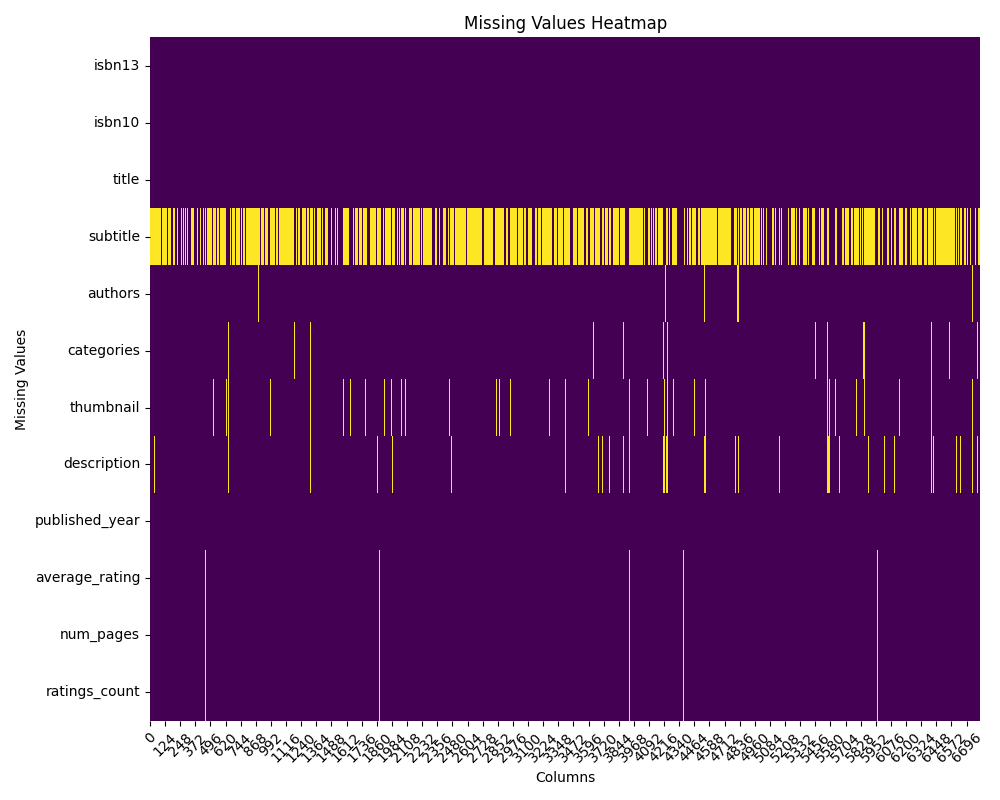
\includegraphics[width=0.9\textwidth]{figures/missing_values_heatmap.png}
    \caption{Missing Values Heatmap: Visualizes the density of missing fields in the original dataset. The heatmap highlights common gaps such as missing subtitles, authors, and thumbnails, prompting the need for augmentation.}
\end{figure}

\begin{figure}[H]
    \centering
    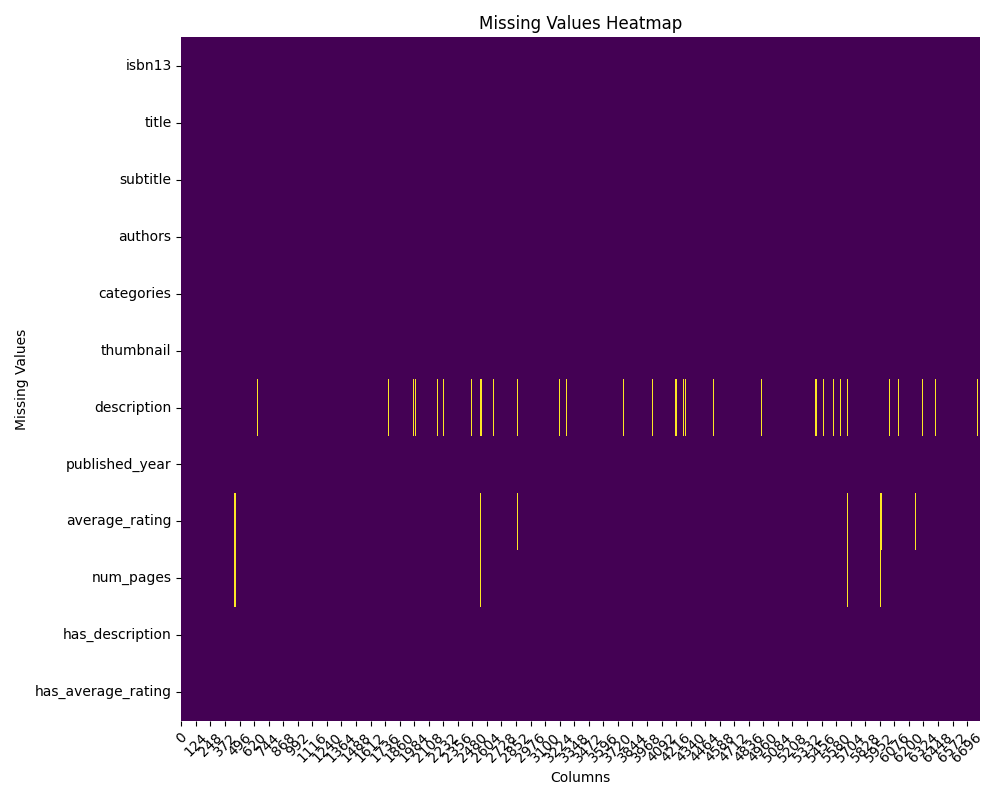
\includegraphics[width=0.9\textwidth]{figures/openlib_values_heatmap.png}
    \caption{OpenLibrary Completion Heatmap: Displays the remaining missing values after OpenLibrary augmentation. It shows improvements in coverage of fields like subtitles, page counts, and published years.}
\end{figure}

\begin{figure}[H]
    \centering
    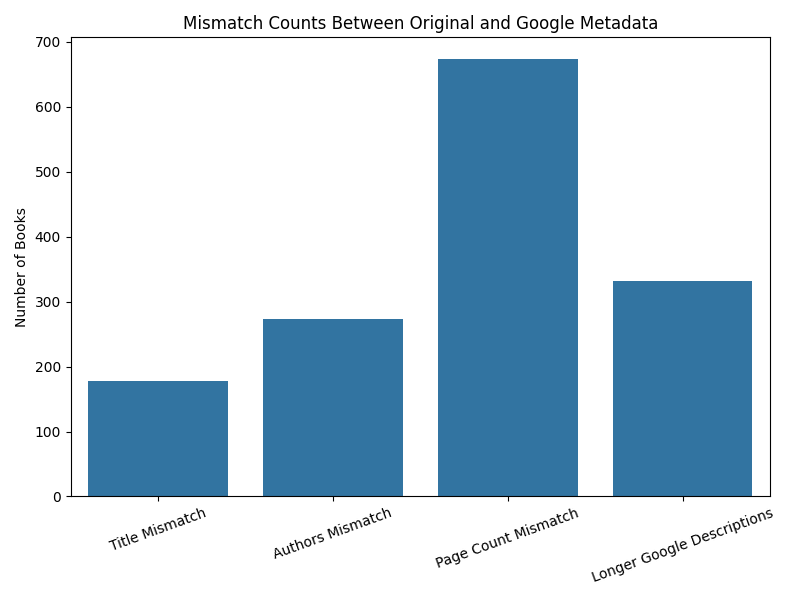
\includegraphics[width=0.9\textwidth]{figures/reexp_mismatch_counts.png}
    \caption{Metadata Conflict Counts: A bar chart showing the number of books with mismatches in title, author, or page count across sources. This justified creation of alternative metadata fields.}
\end{figure}

\begin{figure}[H]
    \centering
    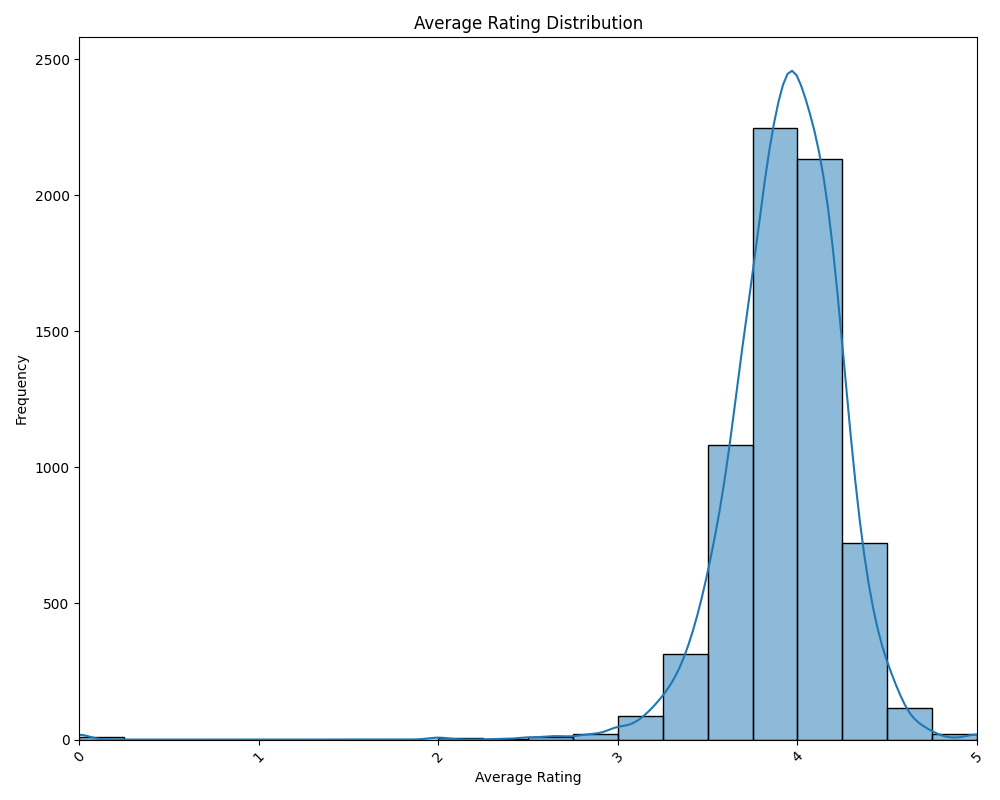
\includegraphics[width=0.9\textwidth]{figures/rating_distribution.png}
    \caption{Rating Distribution: Histogram of average book ratings. The skew toward higher ratings is typical for user-generated content and informed filter default settings.}
\end{figure}

\begin{figure}[H]
    \centering
    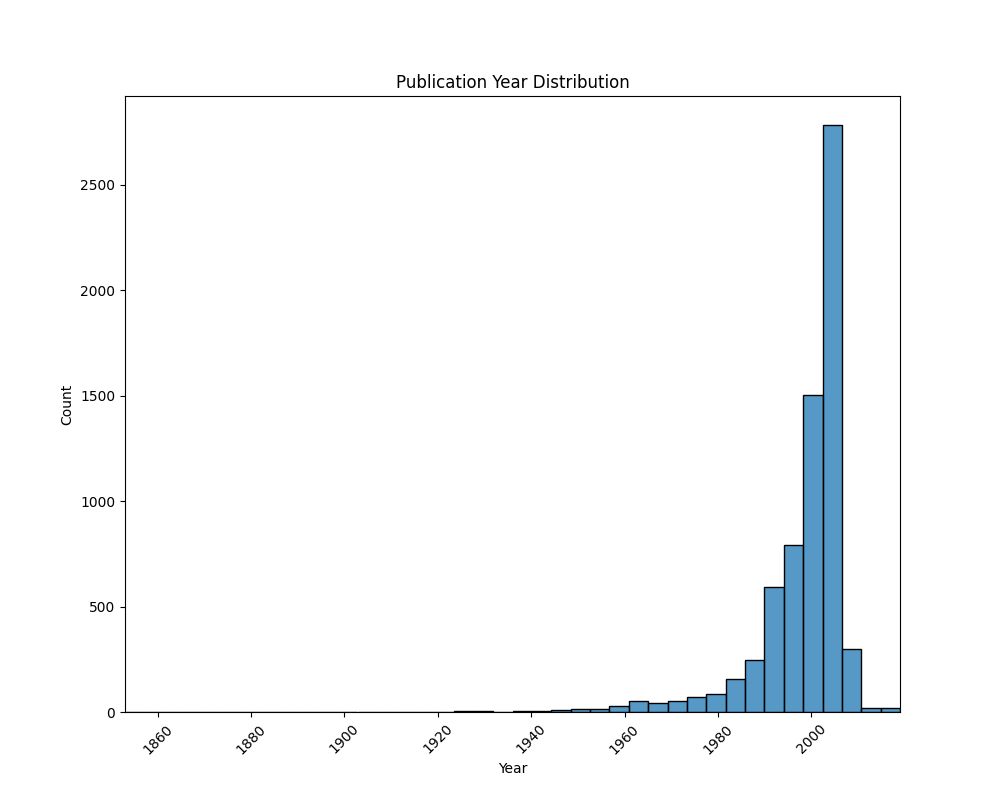
\includegraphics[width=0.9\textwidth]{figures/publication_year_distribution.png}
    \caption{Publication Year Distribution: Shows the number of books published per year. The majority are post-2000, indicating a recency bias that may impact topic coverage.}
\end{figure}

\begin{figure}[H]
    \centering
    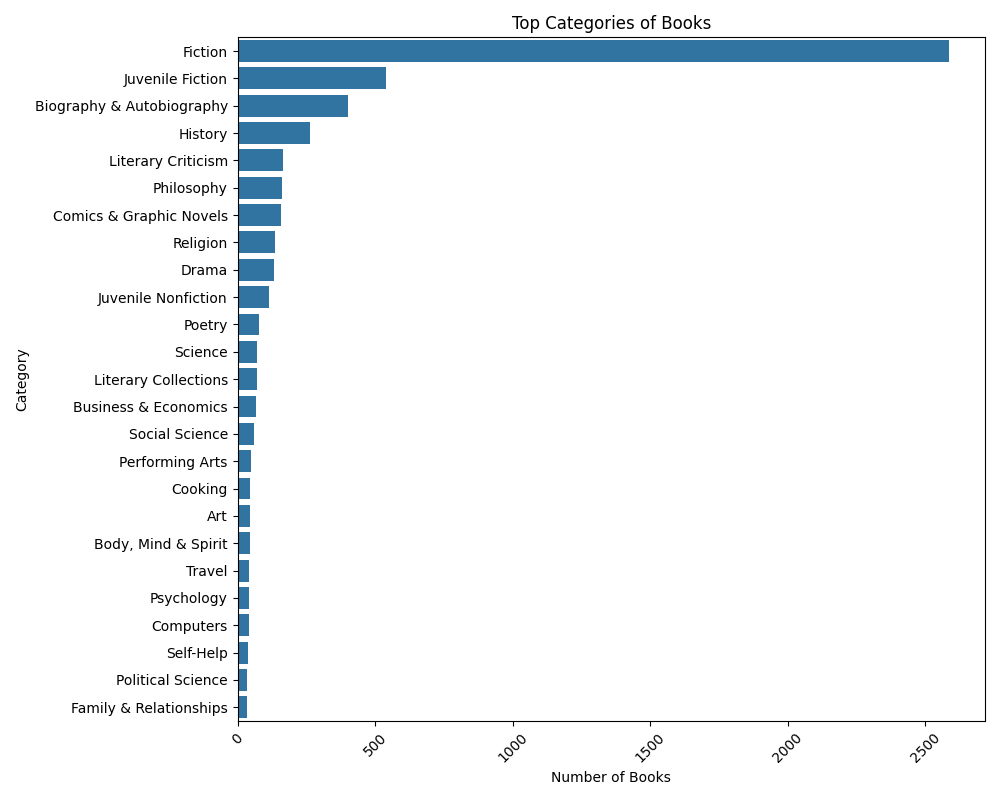
\includegraphics[width=0.9\textwidth]{figures/top_categories.png}
    \caption{Top Categories: A bar chart of the most frequent category labels in the original dataset. This informed the definition of candidate labels for zero-shot classification.}
\end{figure}

\begin{figure}[H]
    \centering
    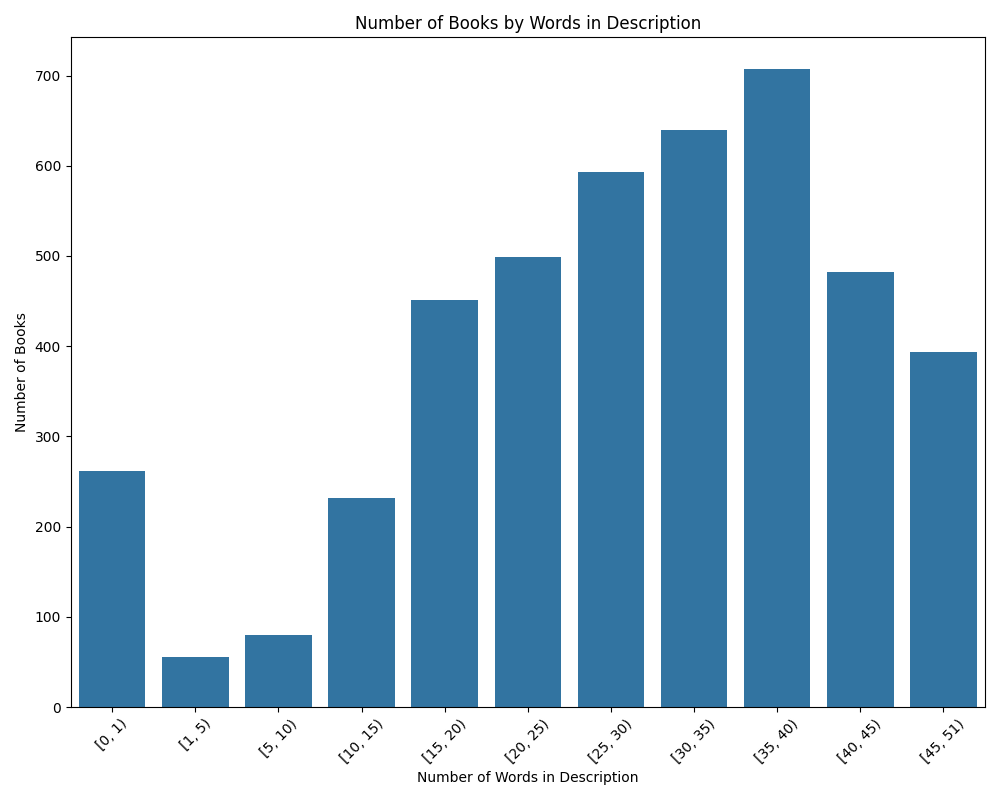
\includegraphics[width=0.9\textwidth]{figures/less_than_50_words_description.png}
    \caption{Books with Short Descriptions: Distribution of books with fewer than 50 words in their descriptions. These entries were flagged for enrichment or removal.}
\end{figure}

\begin{figure}[H]
    \centering
    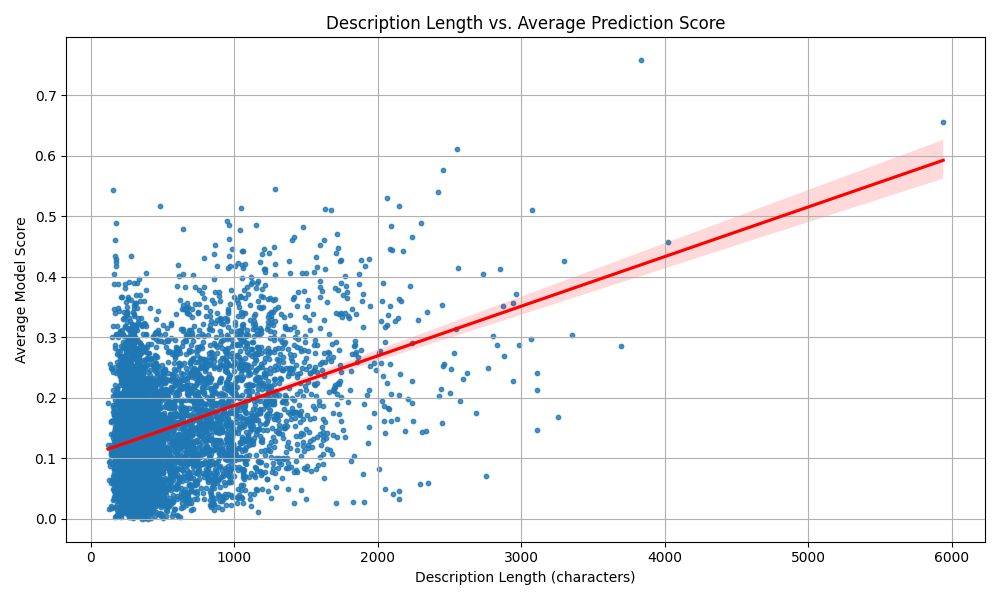
\includegraphics[width=0.9\textwidth]{figures/category_refined_description_length_vs_avg_score.png}
    \caption{Description Length vs. Confidence Score: A regression plot showing the positive correlation between description length and average model confidence. This supported the threshold of 200 characters.}
\end{figure}

\begin{figure}[H]
    \centering
    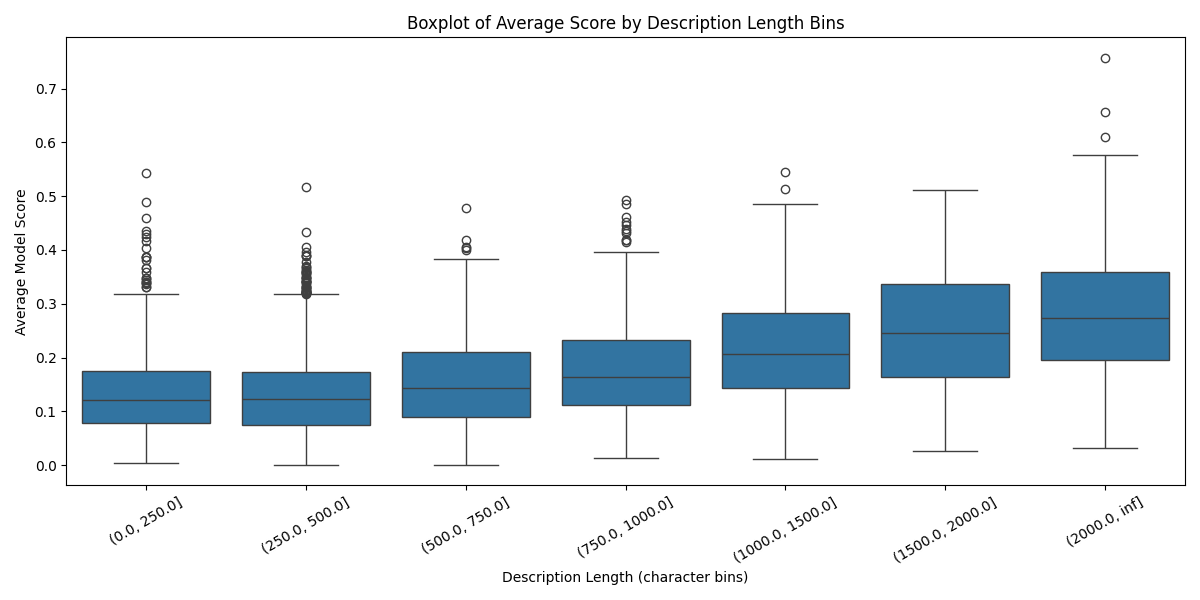
\includegraphics[width=0.9\textwidth]{figures/category_refined_avg_score_by_length_bin.png}
    \caption{Score by Length Bin: A boxplot displaying score variation across binned description lengths. Helps visualize consistency and reliability of model outputs by text richness.}
\end{figure}

\begin{figure}[H]
    \centering
    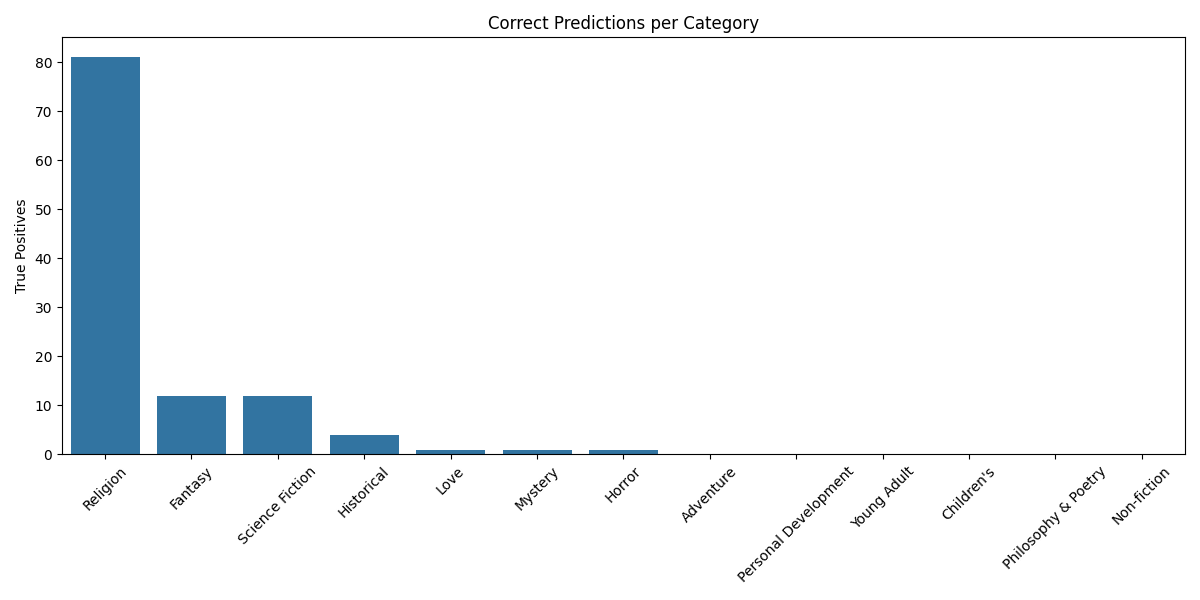
\includegraphics[width=0.9\textwidth]{figures/refine_category_prediction_matches.png}
    \caption{Prediction Matches per Category: Bar chart of true positives per category. Reflects model strength in domains like Fantasy and Love and highlights where fallback logic is critical.}
\end{figure}

% Theoretical Appendices
\chapter{Sentence Embeddings}
\label{appendix:sentence-embeddings}

Sentence embeddings are dense vector representations of entire sentences, designed to capture semantic meaning. Unlike traditional bag-of-words models, embeddings preserve word order and contextual meaning, allowing for nuanced comparisons between texts.

\section*{Intuition}
Where classic keyword-based systems rely on surface matches, sentence embeddings map similar meanings to nearby points in vector space. For instance:

\begin{quote}
\texttt{"A tale of survival in space"}
\end{quote}
\begin{quote}
\texttt{"Story about astronauts facing danger beyond Earth"}
\end{quote}

Though these phrases share few keywords, their embeddings are close in high-dimensional space.

\section*{Transformer-Based Embeddings}
Transformer models such as BERT, RoBERTa, and MiniLM process text using self-attention mechanisms. They generate contextual embeddings — meaning the word \texttt{bank} in "river bank" and "investment bank" will have different vector representations.

Sentence transformers apply pooling strategies (e.g., mean pooling) over token embeddings to produce a single vector per sentence.

\section*{Dimensionality and Use}
In this project, the model \texttt{MiniLM-L6-v2} produces 384-dimensional embeddings:
\[ \vec{v} \in \mathbb{R}^{384} \]
These embeddings are used to:
\begin{itemize}
  \item Represent books (title + description + author)
  \item Represent user queries
  \item Enable similarity search via FAISS
\end{itemize}

\section*{Similarity Metrics}
Cosine similarity and L2 (Euclidean) distance are common metrics. In this system, FAISS uses L2 distance:
\[ \text{dist}(\vec{q}, \vec{b}) = \| \vec{q} - \vec{b} \|_2^2 \]

Smaller distances imply stronger semantic similarity.

\section*{Benefits and Limitations}
\begin{itemize}
  \item \textbf{Pros:} Captures meaning beyond exact words; enables cross-domain generalization; fast inference with MiniLM.
  \item \textbf{Cons:} Embedding quality depends on input quality; short or vague inputs yield weak vectors.
\end{itemize}

\chapter{Zero-Shot Classification}
\label{appendix:zero-shot}

Zero-shot classification is a machine learning technique that allows a model to assign labels to input text without having seen labeled examples for those specific classes. It relies on models trained on general-purpose tasks such as Natural Language Inference (NLI).

\section*{Why Zero-Shot?}
In this project, we did not have human-labeled genres for the books. Instead, we defined a set of target categories (e.g., \textit{Fantasy}, \textit{Science Fiction}, \textit{Historical}) and used a pretrained NLI model to decide whether a description "entails" each candidate label.

\section*{NLI-Based Classification}
The model used was \texttt{facebook/bart-large-mnli}, a transformer trained on premise-hypothesis relationships.

Given:
\begin{itemize}
  \item Premise: the book description
  \item Hypothesis: "This book is \textit{[label]}"
\end{itemize}
The model evaluates whether the hypothesis is entailed by the premise. A high entailment probability means the label is likely correct.

\section*{Multi-Label Inference}
Zero-shot classification supports multi-label predictions. A single description may be associated with multiple categories. Only predictions above a threshold (e.g., 0.4) were retained.

\section*{Advantages}
\begin{itemize}
  \item No training required on project-specific data
  \item Easily extendable to new label sets
  \item Strong generalization using a well-trained NLI base
\end{itemize}

\section*{Limitations}
\begin{itemize}
  \item Performance depends on hypothesis phrasing (e.g., "This book is \textit{fantasy}" vs "This story involves \textit{fantasy}")
  \item May confuse overlapping or abstract categories
  \item Computationally slower than simple keyword matching
\end{itemize}

Zero-shot classification enabled this project to assign interpretable categories to books without manual labeling, supporting both UI filtering and statistical analysis.

\chapter{Similarity Search with FAISS}
\label{appendix:faiss}

Similarity search is the task of finding items most similar to a given query in a high-dimensional vector space. This project uses FAISS (Facebook AI Similarity Search) to perform fast, exact nearest-neighbor lookups over book embeddings.

\section*{Motivation}
Books and queries are embedded into the same semantic vector space. To recommend relevant books, the system retrieves the closest vectors (books) to a given query vector.

\section*{What is FAISS?}
FAISS is a C++/Python library developed by Meta for fast search across large collections of dense vectors. It supports both exact and approximate search methods.

\section*{Indexing Method Used}
This system uses the exact search index:
\begin{itemize}
  \item \texttt{IndexFlatL2} — Computes L2 (Euclidean) distance between the query and all book vectors
  \item Suitable for small to medium datasets (\textasciitilde5,000 vectors)
  \item No compression or quantization
\end{itemize}

\section*{Search Workflow}
\begin{enumerate}
  \item Book metadata is converted to \texttt{search\_text} and embedded
  \item Vectors are added to a FAISS index
  \item At query time, the user input is embedded
  \item FAISS returns top-$k$ nearest neighbors
  \item Metadata is retrieved from the indexed CSV
\end{enumerate}

\section*{Distance Metric}
FAISS computes squared L2 distance:
\[ \text{dist}(\vec{q}, \vec{b}_i) = \| \vec{q} - \vec{b}_i \|_2^2 \]

Lower values indicate higher semantic similarity.

\section*{Benefits}
\begin{itemize}
  \item Extremely fast for exact matching on CPU
  \item Integrates easily with NumPy and PyTorch
  \item Fully offline and open source
\end{itemize}

\section*{Alternatives}
For larger datasets, approximate methods like HNSW, IVF, or PQ (quantization) may be more scalable but require tuning.

FAISS was ideal for this project due to its simplicity and performance at the given scale.
\chapter{Confidence Filtering}
\label{appendix:confidence-filtering}

Confidence filtering is the process of retaining only high-certainty predictions from a model. In this project, it is used to ensure that category labels assigned to books are reliable.

\section*{Motivation}
Zero-shot classification produces a confidence score for each category. However, not all scores are meaningful — low-confidence predictions can lead to noisy or irrelevant labels.

\section*{Metrics Used}
Three metrics were computed for each book's classification output:

\begin{itemize}
  \item \textbf{max\_score} — the highest confidence score among all categories
  \item \textbf{filtered\_avg\_score} — average confidence score for predictions above a threshold (e.g., 0.2)
  \item \textbf{score\_std} — standard deviation of all confidence scores
\end{itemize}

\section*{Filtering Strategy}
To retain high-quality entries for indexing and UI use, books were required to meet all of the following:

\begin{itemize}
  \item \texttt{description\_length} $\geq$ 200 characters
  \item \texttt{filtered\_avg\_score} $\geq$ 0.2
  \item \texttt{max\_score} $\geq$ 0.4
  \item At least one predicted category
\end{itemize}

\section*{Why Multiple Metrics?}
\begin{itemize}
  \item \textbf{max\_score} ensures at least one strong category signal
  \item \textbf{filtered\_avg\_score} avoids noisy averages dominated by low scores
  \item \textbf{score\_std} (analyzed but not thresholded) helps detect ambiguous predictions
\end{itemize}

\section*{Impact}
These thresholds reduced the dataset from 6,572 to 5,160 entries, each with well-supported category labels and semantically rich descriptions. This filtering greatly improved the quality of recommendations.

Confidence filtering balances recall and precision, ensuring that the final indexed dataset is useful and trustworthy.

\chapter{Fallback Classification with Keywords}
\label{appendix:keyword-fallback}

While zero-shot classification captured many semantic categories with high accuracy, some descriptions were too vague or short for the model to assign reliable labels. To compensate, a fallback strategy based on keyword matching was added.

\section*{Motivation}
Some books lack rich descriptions or use metaphoric language. For example, a horror book might avoid directly mentioning "ghosts" or "monsters" but still belong to the genre. Keywords help catch these implicit themes.

\section*{Keyword Lists}
Each predefined category was associated with a curated list of terms. For instance:
\begin{itemize}
  \item \textbf{Fantasy:} \texttt{magic, wizard, dragon, elf, spell}
  \item \textbf{Science Fiction:} \texttt{space, alien, robot, galaxy, dystopia}
  \item \textbf{Love:} \texttt{romance, passion, heartbreak, relationship}
\end{itemize}

These lists were handcrafted and refined iteratively during testing.

\section*{Matching Logic}
After zero-shot prediction:
\begin{itemize}
  \item Each description (or augmented description) was lowercased.
  \item Keyword presence was checked using regular expressions.
  \item Fallback labels were added only if not already predicted by the model.
\end{itemize}

\section*{Benefits}
\begin{itemize}
  \item Increases coverage of categories
  \item Captures under-expressed themes in sparse descriptions
  \item Keeps control in hands of the developer (interpretable logic)
\end{itemize}

\section*{Drawbacks}
\begin{itemize}
  \item Sensitive to phrasing and vocabulary
  \item May overfit to genre stereotypes (e.g., “dragon” always implies Fantasy)
  \item Requires manual tuning and maintenance
\end{itemize}

Fallback classification ensures that every book receives at least one thematic label, improving both UI filter functionality and downstream semantic search quality.

\include{appendix/semantic-vs-keyword}

\end{document}